\documentclass[10pt, xcolor=table]{beamer}

\usepackage[utf8]{inputenc}
\usepackage{amsmath}
\usepackage{amsfonts}
\usepackage{amssymb}
\newcommand*\themecol{\usebeamercolor[fg]{structure}}

\setbeamertemplate{navigation symbols}{}
 \setbeamertemplate{footline}[frame number]



\usepackage{tikz}
\usetikzlibrary{shapes.geometric, arrows}
\tikzstyle{prob} = [rectangle, minimum width=3cm, text width = 4.5cm, minimum height=1cm, text centered, draw=black, fill= blue!20]
\tikzstyle{stat} = [rectangle, minimum width=3cm,  text width = 4.5cm, minimum height=1cm, text centered, draw=black, fill= red!20]
\tikzstyle{arrow} = [thick,->,>=stealth]


\setlength{\parindent}{0pt}
\setlength{\parskip}{6pt}

\title{STAT 111\\
{\small Recitation 2}}

\author{Mo Huang}
\institute{Email: mohuang@wharton.upenn.edu \\
\vspace{0.25cm}
Office Hours: Wednesdays 3:00 - 4:00 pm, JMHH F96\\
\vspace{0.25cm}
Slides: \url{github.com/mohuangx/STAT111-Spring2019} }


\date{February 1, 2019}


\begin{document}

\begin{frame}
\titlepage
\end{frame}



\begin{frame}{The Binomial Distribution: Questions}
\begin{itemize}
\setlength{\itemsep}{15pt}
\item[Q1:] Let $X$ be the number of heads if I toss an unbiased coin 3 times ($n = 3, \theta = 0.5$). Find the probability distribution of $X$ in ``tableau" form.
\item<2->[A1:] \color{red}  
\end{itemize} 
\uncover<2->{ \color{red} {
\begin{columns}
\begin{column}{0.5\textwidth}
\begin{align*}
P(X = 0) &= {3 \choose 0} (0.5)^0 (0.5)^3 \\
&= 0.125 \\
P(X = 1) &= {3 \choose 1} (0.5)^1(0.5)^2 \\
&= 0.375 
\end{align*}
\end{column}
\begin{column}{0.5\textwidth}
\begin{align*}
P(X = 2) &= {3 \choose 2} (0.5)^2(0.5)^1 \\
&= 0.375 \\
P(X = 3) &= {3 \choose 3} (0.5)^3 (0.5)^0 \\
&= 0.125
\end{align*}
\end{column}
\end{columns}}
}

\uncover<3->{ \color{black}
\begin{table}
\begin{tabular}{|c|c|c|c|c|}
\hline
\rowcolor{blue!10} $x$ & 0 & 1& 2&3  \\ \hline
$P(X = x)$ & 0.125 & 0.375 & 0.375 &0.125 \\
\hline
\end{tabular}
\caption{Probability distribution of $X$ using the tableau method.} 
\end{table}}
\end{frame}

\begin{frame}{The Binomial Distribution: Tables}
\begin{itemize}
\setlength{\itemsep}{6pt}
\item[Q2:] $X\sim \mathcal{B}(18, 0.15)$. Find $P(X = 4)$.
\item<2->[A2:] {\color{red} $P(X = 4) = 0.1592$}
\begin{figure}
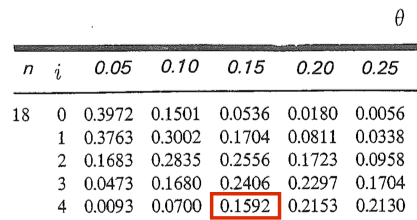
\includegraphics[width = 0.5\textwidth]{images/rec2_1}
\end{figure}
\item<3->[Q3:] Find $P(X \leq 4)$.
\item<4->[A3:] {\color{red} 
\begin{align*}
P(X \leq 4) &= P(X= 0) + P(X=1)+P(X=2)+P(X=3)+P(X=4) \\
&= 0.0536 + 0.1704 + 0.2556 + 0.2406 + 0.1592 \\
&= 0.8794
\end{align*}}
\end{itemize}
\end{frame}

\begin{frame}{The Binomial Distribution: Tables}
\begin{itemize}
\setlength{\itemsep}{6pt}
\item<1->[Q2:] $X\sim \mathcal{B}(12, 0.8)$. Find $P(X = 3)$.
\item<2->[A2:] \color{red} Finding 3 successes with $\theta = 0.8$ is the same as finding 9 failures with $\theta$ of failure $0.2$. Hence, $P(X = 3) = 0.0001$.
\begin{figure}
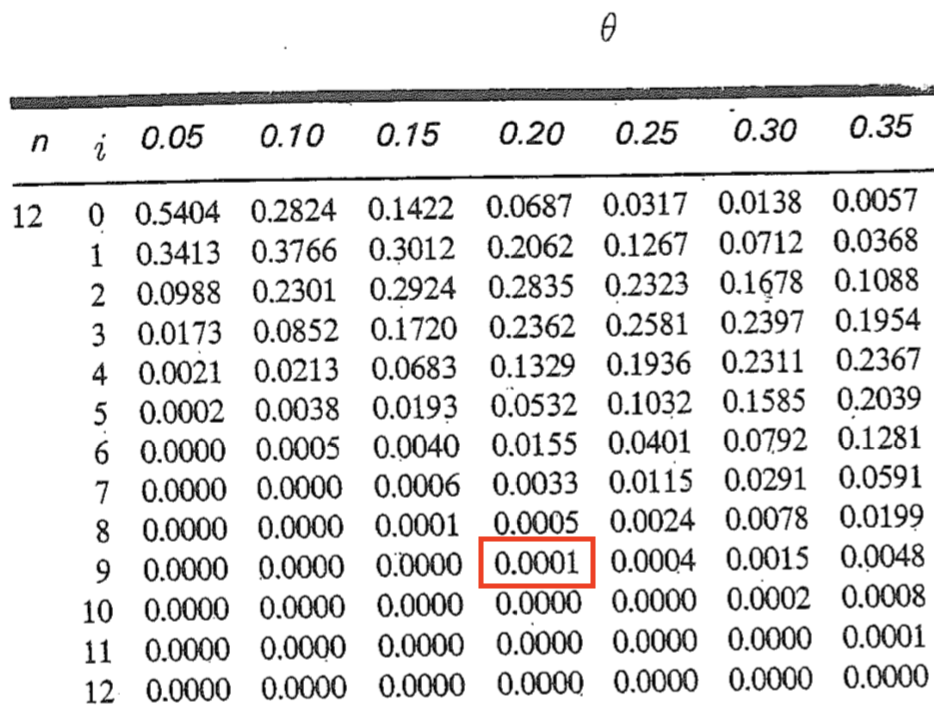
\includegraphics[width = 0.7\textwidth]{images/rec2_2}
\end{figure}
\end{itemize}
\end{frame}


\begin{frame}{Random Variables: Questions}
\begin{itemize}
\setlength{\itemsep}{6pt}
\item[Q2:] Let $X$ be the outcome of one roll of a biased dice where the probability of the number $j$ turning up is $j/21$. Find the mean of $X$.
\item<2->[A2:] {\color{red} \begin{align*}
\mu &= 1 \times 1/21 + 2 \times 2/21 + 3 \times 3/21 + 4 \times 4/21 + 5 \times 5/21 + 6\times 6/21 \\
&= 91/21
\end{align*}}
\vspace{-0.5cm}
\item<3->[Q3:] Let $X$ be a binomial random variable with $n = 2$ and $\theta = 0.8$. Find the mean of $X$ using the binomial table.
\vspace{0.5cm}
\item<4->[A3:] {\color{red} 
\begin{align*}
\mu &= 0 \times 0.04 + 1 \times 0.32 + 2\times 0.64 \\
&= 1.6
\end{align*}}
\vspace{-0.5cm}
\end{itemize}
\end{frame}


\end{document}


